%-------------------------------------------------------------------------------
%                            BAB III
%               		METODOLOGI PENELITIAN
%-------------------------------------------------------------------------------
\fancyhf{} 
\fancyfoot[C]{\thepage}
\chapter{METODOLOGI PENELITIAN}

\section{Waktu dan Lokasi Penelitian}
Penelitian ini akan bertempat pada Gedung A Fakultas Matematika dan Ilmu Pengetahuan Alam. Waktu yang dibutuhkan agar penelitian ini dapat diimplementasikan adalah 4 bulan terhitung dari Juni 2022 hingga September 2022.

\section{Alat dan Bahan}
Alat dan Bahan yang akan digunakan pada penelitian ini terdiri dari beberapa perangkat keras (\textit{Hardware}) dan perangkat lunak (\textit{Software}) yang dijabarkan sebagai berikut:

\begin{enumerate}
\item Perangkat Keras
	\begin{itemize}
	\item Laptop Acer Aspire E5-475g dengan RAM 16GB, Intel Core i5-7200U 2.5GHz, Nvidia GeForce 940MX 2GB, \textit{Harddisk} (HDD) 1500Gb, \textit{Solid State Drive} (SSD) 250GB.
	\item \textit{Smartphone} Xiaomi Poco F3 dengan RAM 6GB, \textit{Internal Storage} 128GB.
	\item \textit{Personal Computer} dengan AMD Ryzen 7 2700x, RAM 16GB, Nvidia GeForce RTX 2080 8GB, \textit{Solid State Drive} (SSD) 500GB.
	\item \textit{Beacon Bluetooth}.
	\end{itemize}

\item Perangkat Lunak
	\begin{itemize}
	\item Windows 11 Pro
	\item Linux Ubuntu 20.04.1 LTS
	\item Android Studio 2021.2.1.15
	\item Visual Studio Code
	\item Figma
	\item Notion
	\item Vosk API
	
	\end{itemize}
\end{enumerate}

\section{\textit{Roadmap} Penelitian}
\textit{Roadmap} penelitian merupakan diagram yang menggambarkan rangkaian beberapa penelitian yang saling berkesinambungan dalam rentang waktu tertentu. \textit{Roadmap} penelitian biasa dibuat untuk memberikan batasan kepada peneliti agar menghindari pengamatan yang tidak perlu dan fokus terhadap bagian penelitiannya saja. Pada penelitian ini dibagi ke dalam 2 fase. Fase pertama pada tahun 2019 memiliki fokus penelitian pada \textit{indoor localization} dengan menggunakan \textit{Bluetooth Low Energy} (BLE) dan menggunakan \textit{Wireless Local Area Network} (WLAN) dapat dilihat gambar \ref{img:fase1}. Pada fase kedua pada tahun 2020 lebih berfokus pada penelitian \textit{Indoor Localization} dengan menggunakan BLE. Penelitian ini terletak pada fase 2 di tahun 2020 dengan topik utama yaitu Aplikasi Navigasi \textit{Indoor} dengan sub topik untuk pengguna Tunanetra. Penelitian ini memiliki batasan berupa pembangunan aplikasi \textit{mobile} untuk \textit{Route Guidance} untuk Tunanetra, seperti yang ditunjukkan pada gambar \ref{img:fase2} dengan kata yang dicetak tebal berwarna merah sebagai berikut.


\begin{figure}[H]
  \begin{adjustbox}{addcode={\begin{minipage}{\width}}{\caption{%
      \textit{Roadmap} Penelitian Fase 1
      }\label{img:fase1}\end{minipage}},rotate=90,center} %label gambar simpen disetelah capt
      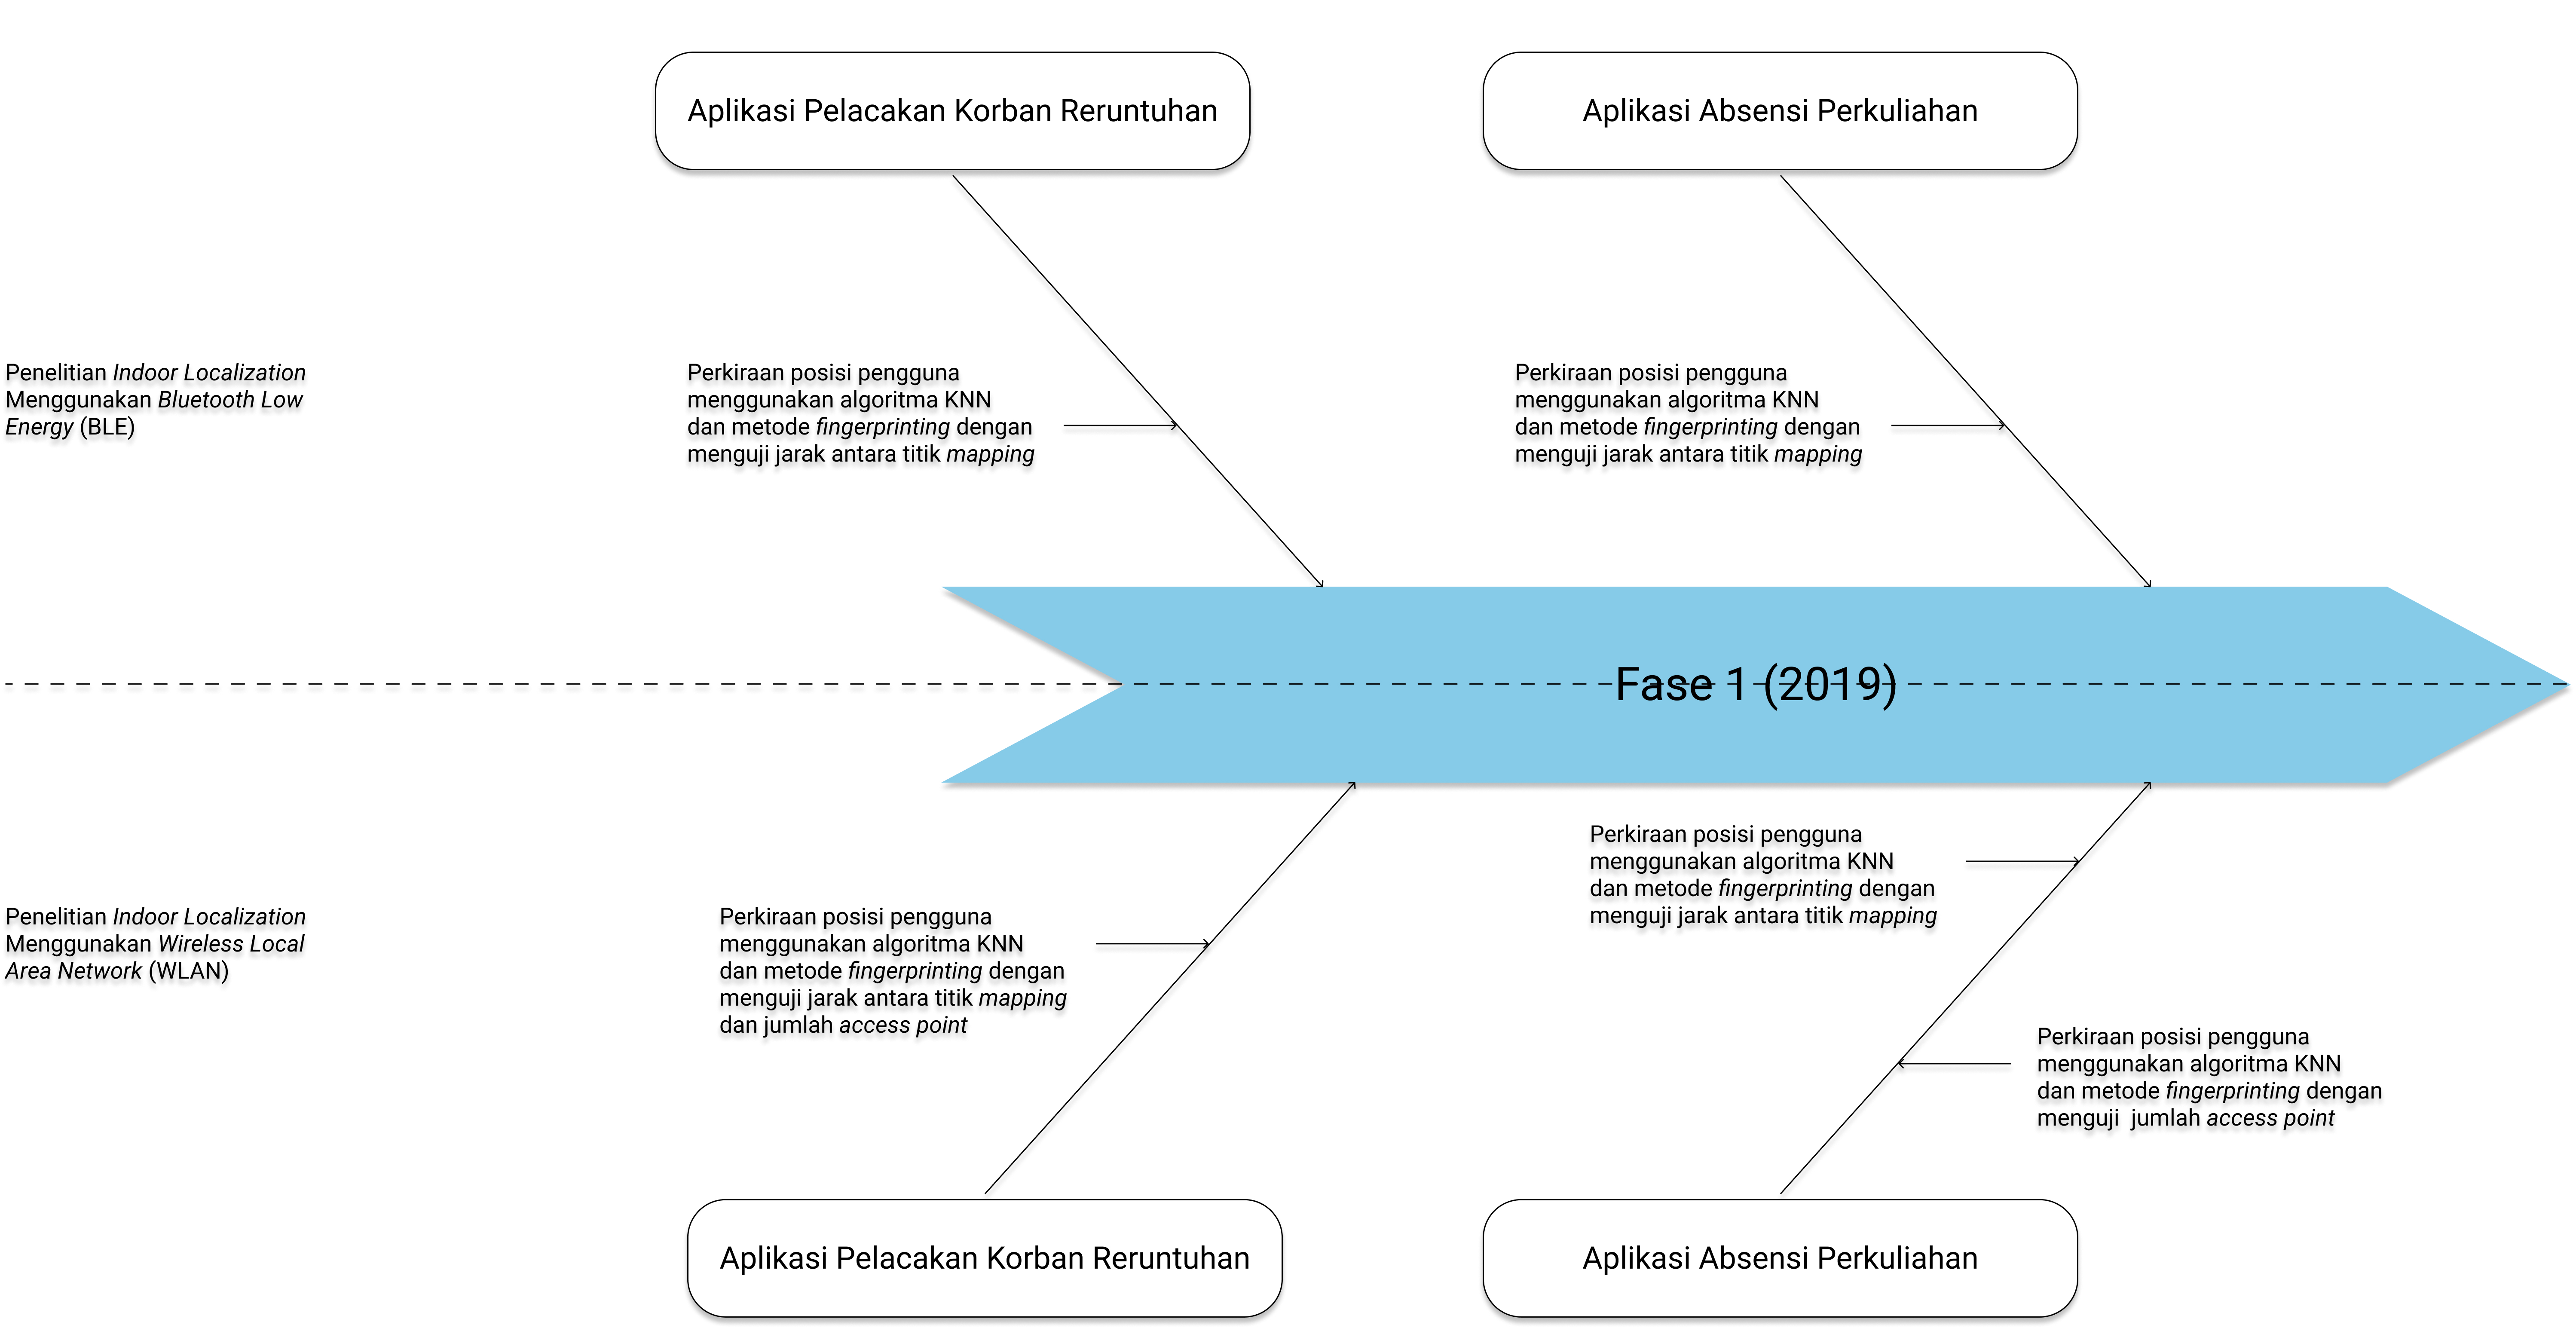
\includegraphics[scale=.3]{gambar/bab3/rp_fase1}%
  \end{adjustbox}
\end{figure}

\fancyhf{} 
\fancyfoot[R]{\thepage}

\begin{figure}[H]
  \begin{adjustbox}{addcode={\begin{minipage}{\width}}{\caption{%
      \textit{Roadmap} Penelitian Fase 2
      }\label{img:fase2}\end{minipage}},rotate=90,center}
      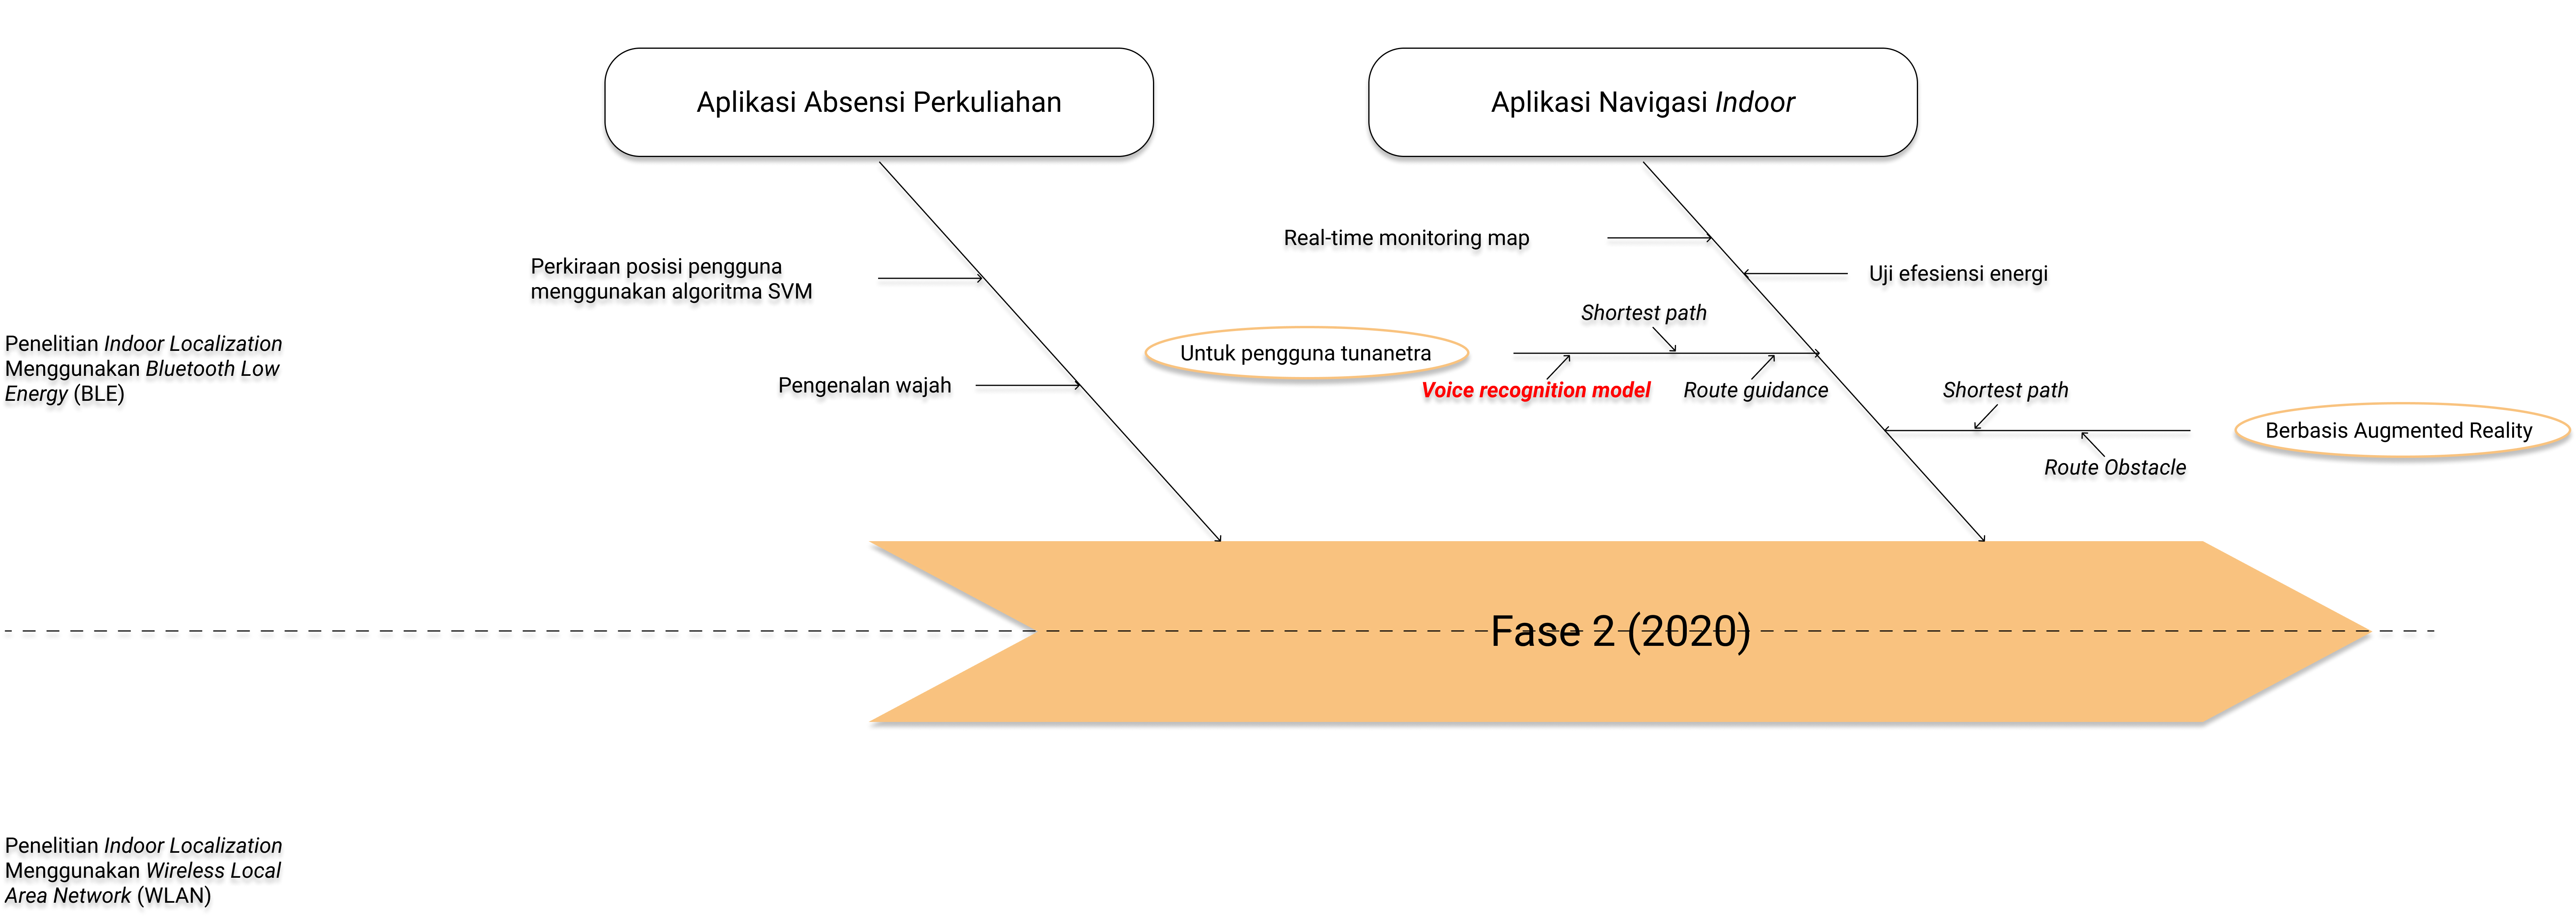
\includegraphics[scale=.3]{gambar/bab3/rp_fase2}%
  \end{adjustbox}
\end{figure}

\fancyhf{} 
\fancyfoot[R]{\thepage}

\section{Metode Penelitian}
Metode penelitian yang dilakukan dalam penelitian ini ditunjukkan pada Gambar \ref{img:diagram_alir_penelitian}.

\begin{figure}[H]
\centering
{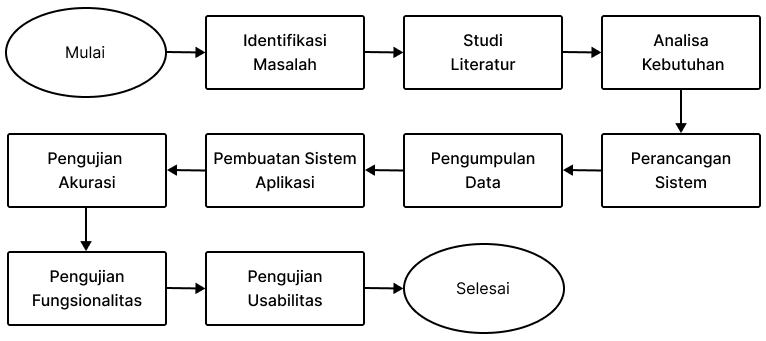
\includegraphics [width = 14cm, height= 8cm]{gambar/bab3/diagram_alir}}
\caption{Diagram Alir Penelitian}
\label{img:diagram_alir_penelitian}
\end{figure}

\fancyhf{} 
\fancyfoot[R]{\thepage}

\subsection{Identifikasi Masalah}
Tahapan ini merupakan tahapan yang dilakukan untuk mengidentifikasi masalah pada lingkungan yang berhubungan dengan aplikasi yang akan dibuat baik secara langsung maupun tidak langsung dan menjadi landasan mengapa aplikasi ini harus dibuat. Masalah-masalah yang berhasil di identifikasi adalah sebagai berikut:

\begin{enumerate}
\item Kebutuhan Fungsional
Kebutuhan fungsional mendefinisikan fungsionalitas sistem. Kebutuhan fungsional dari identifikasi masalah yang telah dilakukan adalah sebagai berikut:

\begin{itemize}
\item Melakukan proses pemanduan kepada pengguna secara background process dengan bantuan \textit{speech command recognition} dan \textit{route guidance} dengan aplikasi berbasis Android.

\item Menampilkan prediksi lokasi pengguna serta rute terbaik menuju ke lokasi tujuan pengguna.

\end{itemize}

\item Kebutuhan Non-Fungsional
Kebutuhan non-fungsional memastikan batasan eksternal yang harus dipenuhi oleh sistem. Batasan-batasan tersebut antara lain:

\begin{itemize}
\item Proses pemanggilan aplikasi dimulai dengan memanggil \textit{hotword}.

\item Proses pencatatan dan penentuan lokasi dilakukan secara berkala dalam interval yang sesingkat-singkatnya.

\item Hanya dapat melakukan proses pemanduan rute apabila \textit{Bluetooth} pada perangkat hidup dan terhubung dengan \textit{Beacon}.

\item Sistem hanya dapat mendeteksi lokasi pengguna di dalam gedung yang telah di petakan terlebih dahulu.

\end{itemize}

\end{enumerate}

%%%%%%%%%%%%%%%%%%%%%%%%%%%%%%%%%%%%%%%%%%%
\subsection{Studi Literatur}
Studi literatur digunakan sebagai bahan referensi selama proses penelitian. Studi literatur dilakukan dengan cara mencari situs \textit{website} dan jurnal-jurnal terkait tentang penelitian, baik jurnal nasional maupun internasional, buku-buku yang telah diterbitkan, serta situs-situs internet yang berkaitan dengan permasalahan yang dikaji dalam penelitian. Studi literatur dapat dikembangkan untuk menyempurnakan kekurangan dari penelitian sebelumnya.

%%%%%%%%%%%%%%%%%%%%%%%%%%%%%%%%%%%%%%%%%
\subsection{Perancangan Sistem}
Tahap perancangan sistem ini meliputi perancangan alur kerja sistem yang berfungsi untuk memastikan sistem yang dibangun dapat digunakan secara baik oleh pengguna. Tahap perancangan sistem ini terbagi menjadi beberapa bagian yaitu diagram Use Case , Diagram Deployment, alur kerja sistem, dan desain prototipe berdasarkan analisa kebutuhan yang telah dijabarkan. Berikut ini merupakan tahapan tersebut:



\begin{enumerate}
\item \textit{Use Case Diagram}
\par \textit{Use Case Diagram} merupakan gambaran interaksi antara pengguna dan sistem. Pengguna dari sistem yang akan dibangun ini adalah Tunanetra dan pengunjung gedung FMIPA USK. \textit{Use Case Diagram} dari sistem ini dapat dilihat pada Gambar \ref{img:use_case_diagram}

\begin{figure}[H]
\centering
{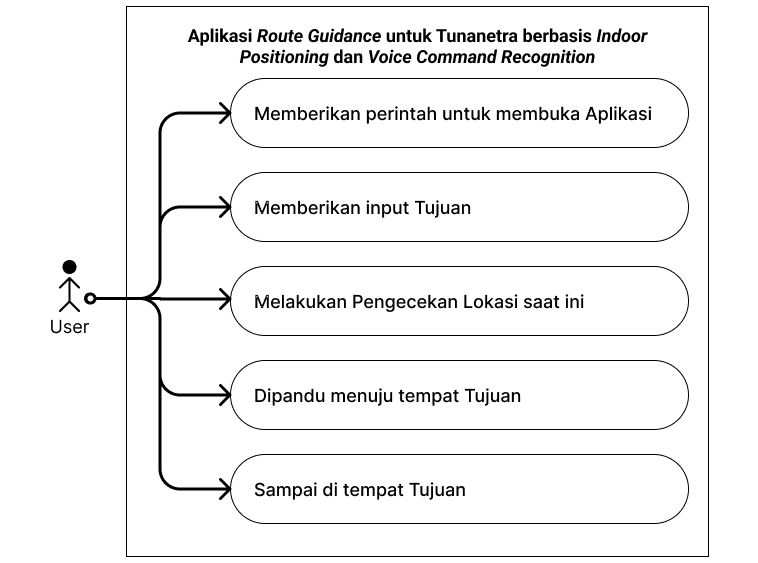
\includegraphics [width = 14cm, height= 12cm]{gambar/bab3/use_case_diagram}}
\caption{\textit{Use Case Diagram}}
\label{img:use_case_diagram}
\end{figure}


\item \textit{Deployment Diagram}
\par \textit{Deployment Diagram} merupakan gambaran hubungan antara perangkat lunak dan perangkat keras yang digunakan dalam sebuah sistem. Seperti yang telah disebutkan sebelumnya, penelitian ini merupakan bagian dari penelitian lain yang saling terintegrasi sehingga tidak semua \textit{node} dalam diagram menjadi fokus dalam penelitian ini. Bagian dalam diagram yang menjadi jangkauan dari penelitian ini ditandai dengan warna biru seperti yang ditunjukkan pada Gambar \ref{img:use_case_diagram}

\begin{figure}[H]
\centering
{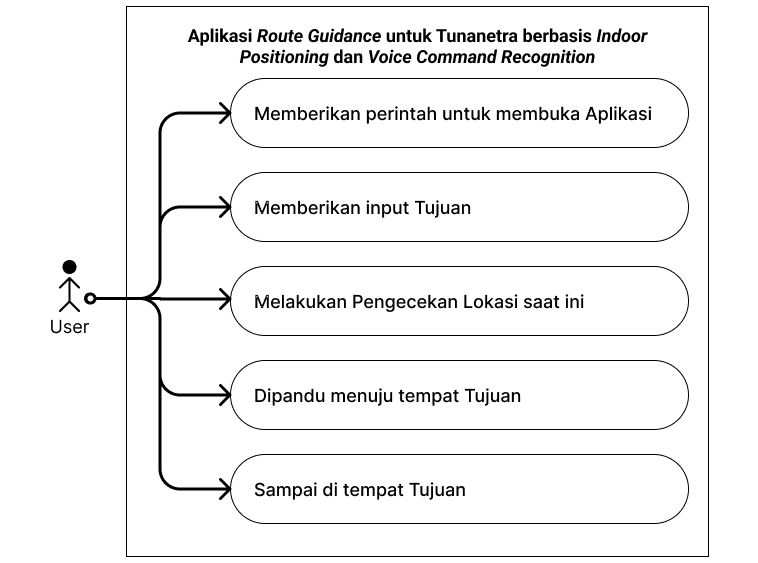
\includegraphics [width = 14cm, height= 12cm]{gambar/bab3/use_case_diagram}}
\caption{\textit{Use Case Diagram}}
\label{img:use_case_diagram}
\end{figure}

\end{enumerate}

%%%%%%%%%%%%%%%%%%%%%%%%%%%%%%%%%%%%%%%%%

\subsection{Alur Kerja Sistem}
Alur kerja sistem merupakan langkah-langkah yang dilalui sistem hingga fungsionalitas sistem dapat dimanfaatkan oleh pengguna. Alur kerja sistem ini dapat dilihat pada Gambar \ref{img:alur_kerja_sistem}

\begin{figure}[H]
\centering
{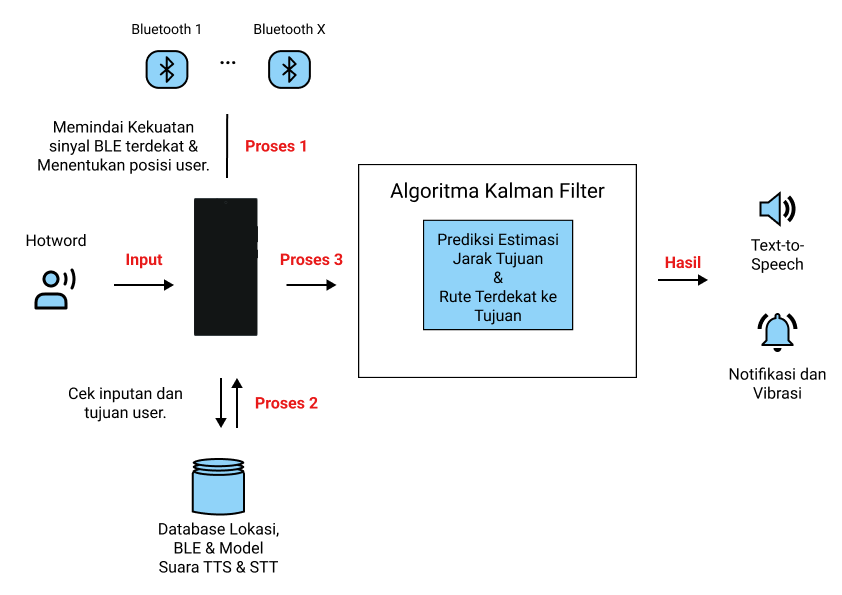
\includegraphics [width = 14cm, height= 10cm]{gambar/bab3/alur_kerja_sistem}}
\caption{Alur Kerja Sistem}
\label{img:alur_kerja_sistem}
\end{figure}


\subsection{Akustik Model}
Pada bagian ini merupakan tahapan untuk melakukan model akustik pada data training yang telah melewati proses ekstraksi fitur dengan MFCC. Tahapan ini menggunakan proses \textit{machine learning} dengan metode \textit{Deep Neural Network} (DNN) dan dilakukan juga pengambilan nilai \textit{CTC Loss} yang merepresentasikan akurasi dari \textit{training}. Pada tahap awal \textit{training} dimulai dengan menentukan jumlah \textit{file} yang masuk ke dalam perhitungan ke \textit{deep learning} sebagai bahan dari pembelajaran atau pembagi data. Setelah itu nilai dari MFCC \textit{feature} dimasukkan, lalu label untuk proses pembelajaran dimasukkan juga. Berikutnya dilakukan inisialisasi \textit{learning rate}, maksimal \textit{epoch} dan minimum \textit{loss} yang digunakan. Lalu pada proses perhitungan \textit{neural network} diinisialkan bobot yang dipakai. Selanjutnya metode \textit{deep learning} dengan \textit{input} nilai MFCC \textit{feature} dan target dihitung. Terakhir menampilkan nilai \textit{loss} dari hasil perhitungan yang didapat. Hal tersebut dilakukan sampai mendapatkan minimum nilai \textit{loss} dan maksimum nilai \textit{epoch}. Pada penelitian ini digunakan \textit{multilayer perseptron} sebagai layer pembelajarannya. 

\subsection{Model}
Setelah mendapatkan hasil dari \textit{acoustic modelling} dengan Kaldi, selanjutnya melakukan \textit{language modelling} dengan menggunakan SRILM (\textit{SRI Language Modeling Toolkit}). \textit{Language modelling} berguna agar dapat membedakan kata dan frasa yang terdengar serupa pada ucapannya sehingga didapatkan model pengenalan ucapan yang terlatih. 

\subsection{Model Terlatih}
Setelah model pengenalan ucapan sudah selesai dibangun, lalu model tersebut diletakan pada Vosk yang merupakan \textit{open source speech recognition toolkit}, Vosk dapat berjalan pada Android dengan API secara \textit{offline}. Data \textit{testing} yang sebelumnya sudah dipisahkan, diuji pada model tersebut sehingga mendapatkan keluaran berupa \textit{text}. Model ini akan dapat berjalan pada aplikasi Android \textit{route guidance} untuk tuna netra berbasis \textit{Indoor Positioning} yang akan dibangun.

%-----------------------------------------------------------------------------%

% Baris ini digunakan untuk membantu dalam melakukan sitasi
% Karena diapit dengan comment, maka baris ini akan diabaikan
% oleh compiler LaTeX.
\begin{comment}
\bibliography{daftar-pustaka}
\end{comment}